%Notes by Harsh Mistry 
%Econ 301
%Based on Template From  https://www.cs.cmu.edu/~ggordon/10725-F12/template.tex

\documentclass[twoside]{article}
\setlength{\oddsidemargin}{0.25 in}
\setlength{\evensidemargin}{-0.25 in}
\setlength{\topmargin}{-0.6 in}
\setlength{\textwidth}{6.5 in}
\setlength{\textheight}{8.5 in}
\setlength{\headsep}{0.75 in}
\setlength{\parindent}{0 in}
\setlength{\parskip}{0.1 in}
\usepackage{amsmath,amsfonts,graphicx, color}
\newcounter{lecnum}
\renewcommand{\thepage}{\thelecnum-\arabic{page}}
\renewcommand{\thesection}{\thelecnum.\arabic{section}}
\renewcommand{\theequation}{\thelecnum.\arabic{equation}}
\renewcommand{\thefigure}{\thelecnum.\arabic{figure}}
\renewcommand{\thetable}{\thelecnum.\arabic{table}}
\newcommand{\lecture}[4]{
   \pagestyle{myheadings}
   \thispagestyle{plain}
   \newpage
   \setcounter{lecnum}{#1}
   \setcounter{page}{1}
   
   
%Info Box 
   \begin{center}
   \framebox{
      \vbox{\vspace{2mm}
    \hbox to 6.28in { {\bf Econ 301 - Microeconomic Theory 2
	\hfill Winter 2018} }
       \vspace{4mm}
       \hbox to 6.28in { {\Large \hfill Lecture #1: #2  \hfill} }
       \vspace{2mm}
       \hbox to 6.28in { {\it Lecturer: #3 \hfill Notes By: #4} }
      \vspace{2mm}}
   }
   \end{center}
   
   \markboth{Lecture #1: #2}{Lecture #1: #2}



 
}

\renewcommand{\cite}[1]{[#1]}
\def\beginrefs{\begin{list}%
        {[\arabic{equation}]}{\usecounter{equation}
         \setlength{\leftmargin}{2.0truecm}\setlength{\labelsep}{0.4truecm}%
         \setlength{\labelwidth}{1.6truecm}}}
\def\endrefs{\end{list}}
\def\bibentry#1{\item[\hbox{[#1]}]}

\newcommand{\fig}[3]{
			\vspace{#2}
			\begin{center}
			Figure \thelecnum.#1:~#3
			\end{center}
	}
	
	\graphicspath{ {images/} }

\newtheorem{theorem}{Theorem}[lecnum]
\newtheorem{lemma}[theorem]{Lemma}
\newtheorem{ex}[theorem]{Example}
\newtheorem{proposition}[theorem]{Proposition}
\newtheorem{claim}[theorem]{Claim}
\newtheorem{corollary}[theorem]{Corollary}
\newtheorem{definition}[theorem]{Definition}
\newenvironment{proof}{{\bf Proof:}}{\hfill\rule{2mm}{2mm}}
\newcommand\E{\mathbb{E}}


%Start of Document 
\begin{document}

\lecture{4}{January 15, 2018}{Jean Guillaume Forand}{Harsh Mistry}
\section{Consumer Choice Continued}
\begin{itemize}
\item We often impose additional assumptions on preferences to yield "nice" (201) indifference curves
\end{itemize}
\begin{definition}
The preference relation \(\succeq\) on \(\mathbb{R}^2_+\) is 
\begin{enumerate}
\item \underline{Monotone} if for all \(x, y \in \mathbb{R}^2_+\) such that \( x_1 > y_1\) and \(x_2 > y_2\). We have that \(x \succ y \)
\item \underline{Convex} if for all \(x, y \in \mathbb{R}^2_+\) such that \(x \sim y \) and for all \( 0 \leq \alpha \leq 1 \). We have that \( \alpha x + (1 - \alpha) y geq x\) 
\end{enumerate}
\end{definition}

\begin{itemize}
\item Monotonicity states that bundles containing strictly more goods are strictly preferred by the consumer
\begin{itemize}
\item This rules out "thick" indifference curves
\end{itemize}
\item Convexity ensures "nicely" curved indifference curves. 
\begin{itemize}
\item Represents a preference for diversity
\item States that mixture of bundles never make the consumer worse off
\end{itemize}
\item Indifference curves that violate convexity : 
\begin{center}
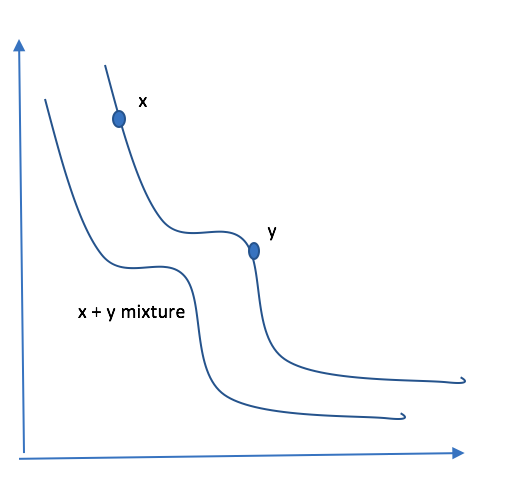
\includegraphics[scale=0.35]{7}
\end{center}
\item Convexity assumptions induce convenient properties in consumers optimisation problem 
\begin{itemize}
\item Ensures that sufficient or "second-order" conditions are satisfied
\end{itemize}
\end{itemize}

\subsection{Utility}
\textbf{\textcolor{red}{In class numbering : 1.1.4}}
\begin{itemize}
\item A utility function is a \underline{tool} for representing preference relations.
\end{itemize}

\begin{definition}
A function \(u : \mathbb{R}_+^2 \rightarrow \mathbb{R} \) is a \underline{utility function representing preference relation} \(\succeq\) if for all \(x, y \in \mathbb{R}^2_+\)
\[ u(x) \leq u(y) \iff x \succeq y\]
\end{definition}
\begin{itemize}
\item Note that \(u(x) > u(y) \iff x \succ y\) and \(u(x) = u(y) \iff x \sim y \)
\item "Utility" is not some physical quantity. Meaning is attached to utility numbers only in so that they allow us to reconstruct preference statements 
\end{itemize}

\begin{ex}
Suppose that goods 1 and 2 are \underline{perfect substitutes}
\[ x \succeq y \iff x_1 + x_2 \geq y_1 + y_2\]
\begin{center}
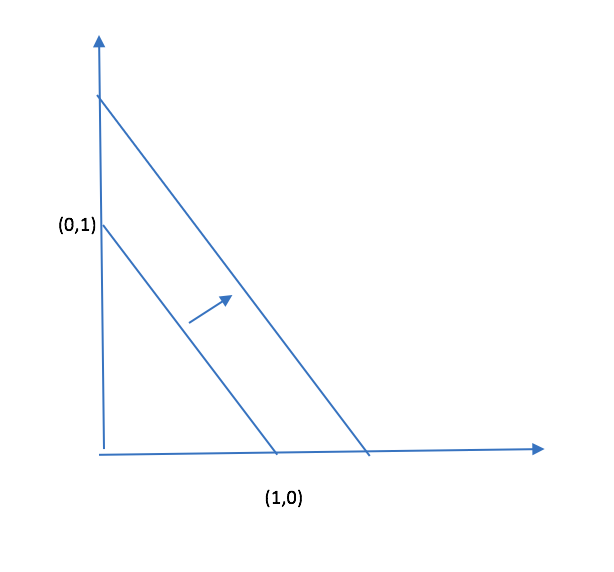
\includegraphics[scale=0.4]{8}
\end{center}
\(u(x_1, x_2) = x_1 + x_2\) is a utility function representing \(\succeq\), but so is \(u(x_1, x_2) = ln((x_n + x_2)^2) + 36\)
\end{ex}

\begin{itemize}
\item Any transformation of utility numbers that maintains their order which represents the same preference relation
\item Consider a strictly increasing function \[f : \mathbb{R} \rightarrow \mathbb{R}_+. then f(u(x)) \geq f(u(y)) \iff u(x) geq u(y) \iff x \succeq y \]
So that \(f(u(\cdot))\) is a utility function representing \(\succeq\)
\item Utility functions represent the \underline{ordinal} information contained in preferences
\item Important question : Can any preference relation be represented by a utility function. 
\begin{itemize}
\item No if preferences are not complete. \\
\textbf{Proof By contradiction : } suppose not \(x \succeq y \) and not \(y \succeq x\), but u represents \(\geq\). Then either  Contradiction \(u(x) \geq u(y)\) or \(u(y) \geq u(x)\) or \(u(x) \geq u(y)\), thus \(x \succeq y\) or \(y \succeq x\). Contradiction.
\item No if preferences are not transitivity
\item Yes if preferences are complete, transitive, and satisfy additional continuity assumptions 
\end{itemize}
\end{itemize}

\subsection{Optimal consumer choice}
\textbf{\textcolor{red}{In class numbering : 1.1.5}}
\begin{itemize}
\item Consumers choice problem has been reduced to constrained optimization problem: 
\[max_{x_1, x_2 \geq 0} \hspace{0.1cm} u(x_1, x_2)  \text{ subject to } p_1 x_1 +  p_2 x_2 \leq m \]
\end{itemize}

\end{document}





